\documentclass[12pt, preprint]{aastex}
\usepackage{amsmath}
\usepackage{natbib}

\def\PS  {\hbox{Pan-STARRS}}
\def\RR  {\hbox{RR Lyrae}}


\begin{document}
\title{A pilot study of the Pan-STARRS potential for finding RR Lyrae}
\slugcomment{August 28, 2014}
\author{The MPIA Summer 2014 RR Lyrae Tiger Team}
 

\begin{abstract}
We used variable \PS\ sources from the SDSS Stripe 82 region, together with WISE
photometry, to select a sample of candidate \RR. Aided by a sample of known
\RR\ with SDSS-based template light curves, we used template-fitting method
and estimated its sample completeness and purity. Our results motivate 
the application of this method to the whole sky region covered by \PS. 
\end{abstract}


\section{Introduction}

Pan-STARRS data have the potential to extend the faint limit for finding \RR\ stars by about 
a magnitude, compared to the deepest available datasets. For motivation why to 
search for \RR, relevant references, and an attempt to find \RR\ in \PS, see
Abbas et al. (2014, AJ 148, 8). 

Abbas et al. used SDSS colors (because they are nearly simultaneously measured)
and \PS\ variabiltiy estimators to select candidate \RR. They achieved completeness
of 52\% and purity (100\% minus ``contamination'') of 77\% (measured using a known sample 
of \RR\ from SDSS Stripe 82). Most of their contaminants are stars rather than quasars 
because the latter were efficiently rejected using the SDSS $u-g$ color. Therefore,
this performance characteristics {\bf cannot} be obtained over the entire \PS\ footprint
(about twice as large as covered by SDSS) due to the lack of SDSS $u$ band measurements. 

The only variability information that Abbas et al. used is a simple cut on the 
root-mean-square variability in the \PS\ $i_P$, $z_P$ and $y_P$ bands, with
at least three detections in each band. In particular, they did not attempt to fit 
\RR\ light curve templates to \PS\ data.  Light-curve template fitting can improve the 
selection of \RR\ in \PS\ because of more information being used in the process. 
Furthermore, if the improvement is significant, it might be possible to abandon 
selection cuts based on SDSS data and thus extend the search to the full \PS\ 3$\pi$ area.
Investigating this possibility was the main aim of this pilot study. 




\section{Pilot Study} 


We first discuss the selection of candidate \RR\ using \PS\ and WISE data, and then 
discuss the results of applying the template fitting method to selected candidates. 


\subsection{Selection of candidate \RR\ using \PS\ and WISE data} 

The final step of the selection algorithm operates in a 4-dimensional space spanned
by WISE $W1-W2$ color (3.4 $\mu$m $-$ 4.6 $\mu$m), \PS\ $g-r$ color and \PS\ 
based variability parameters $q$ (statistical significance of the observed variability)
and $\tau$ (time scale for a damped random walk fit, in days). Prior to this step, a 
number of quality cuts are performed by Nina's code, as explained in her document.
In addition to quality cuts, Nina also places a cut on $q$, the statistical significance 
of the observed variability ($q=\chi^2_{dof} \, \sqrt{N_{dof}/2}$), and fits damped random 
walk model to all candidate sources. Nina's quality cuts are by and large driven by the 
quantity and quality of available \PS\ data, and together with the $q>5$ cut, result in a
 {\bf starting selection completeness of about 75\%.}  Only 7.5\% of all selected
sources are confirmed \RR\ (purity=7.5\%). The following cuts were used to significantly 
increase sample purity, while maintaining relatively high completeness. 

Based on the behavior of known \RR\ and quasars (361 and 2373, respectively, 
out of 4831 selected sources), illustrated in Fig.~\ref{Fig:selection}, the following 
selection cuts were adopted (in addition to the general $14 < g < 21$ requirement): 
\begin{enumerate}
\item $-1.0<g-r<0.4$ to reject red sources. 
\item $q>30$ to reject small-amplitude variables.
\item $\tau < 10$ days to reject most quasars and long-period variables.
\item $W1-W2 < 0.5$ (when detected by WISE)  to reject essentially all quasars. 
\end{enumerate} 

These selection criteria result in a sample completeness of 75\% (overall 50\%, since
Nina's selection had a completeness of, coincidentally, 75\%) and purity of 50\%. 
Selection by colors only results in completeness of 85\% and purity of 24\%,
and selection by variability results in completeness of 89\% and purity of 35\%.
Most of contaminants are expected to be eclipsing binary stars from the blue
end of the main stellar locus. Quasars are not expected to represent a major
contaminant: just like Abbas et al. rejected them using SDSS $u-g$ colors,
here we rejected them using WISE $W1-W2$ colors. 

Therefore, instead of attempting light curve fitting for 4831 sources that include
361 \RR\, now we can fit 539 light curves that include 269 \RR\ (an incremental loss 
of 25\% of \RR), while decreasing the initial sample by a factor of 9. 


\begin{figure}[!t]
\vskip -1.5in
\hskip -0.13in
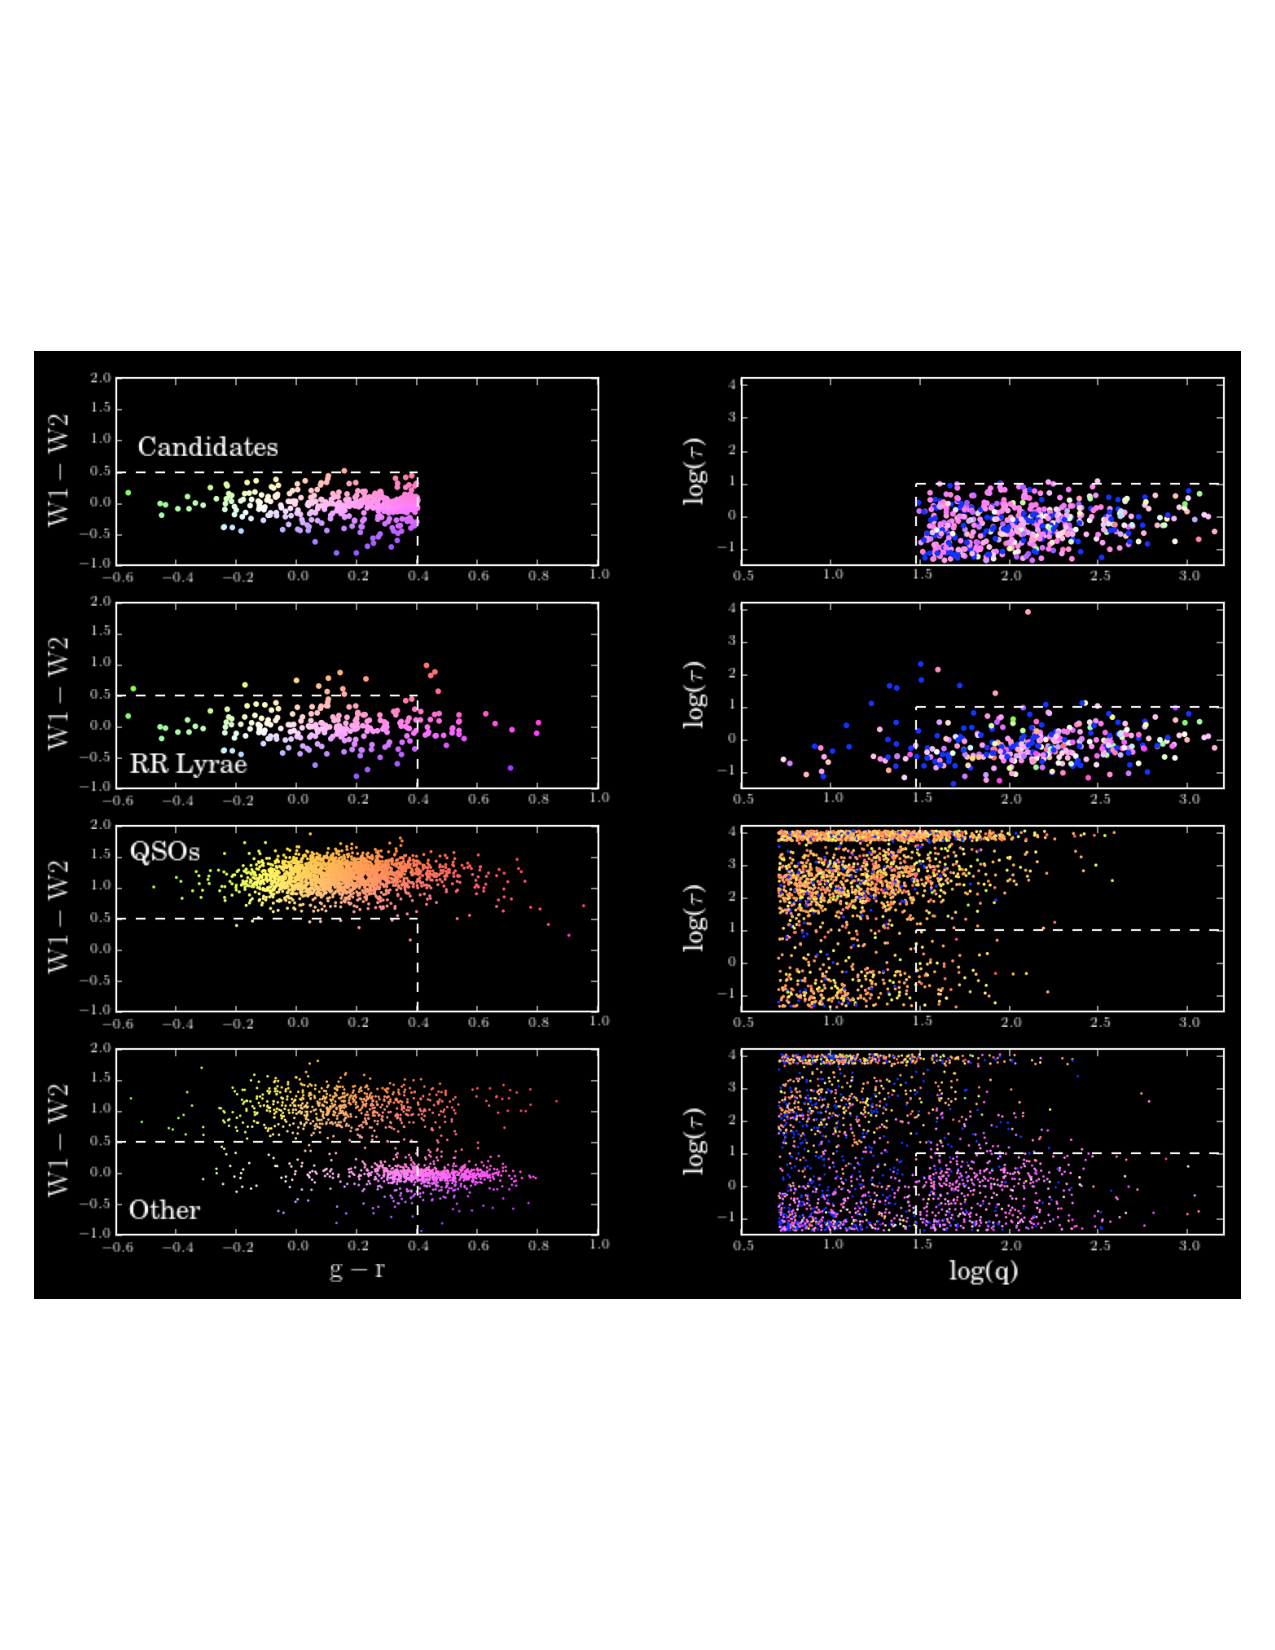
\includegraphics[width=1.05\hsize,clip]{plotSelection.pdf}
\vskip -1.7in
\caption{Summary of the selection procedure based on WISE $W1-W2$ color (3.4 $\mu$m $-$ 4.6 $\mu$m)
\PS\ $g-r$ color and \PS\ based variabilty parameters $q$ (statistical significance of the observed variability)
and $\tau$ (time scale for a damped random walk fit, in days). The left column shows the $W1-W2$ vs. $g-r$
color-color diagram and the right column shows the $\log(\tau)$ vs. $q$ ``variability'' diagram for sources
from the SDSS Stripe 82 region. The symbols are color-coded in 2 dimensions, according to their position in 
the color-color diagram (the blue symbols in the variability diagram for \RR\ are objects without WISE detections;
practically all quasars are detected by WISE). 
The known \RR\ and quasars are shown in the second and third row, and unclassified sources are shown in the 
bottom row. The white dashed lines show the adopted selection boundaries for \RR\  based on the behavior of 
known \RR\ and quasars. The top row shows the selected candidate \RR.} 
\label{Fig:selection}
\end{figure}



\subsection{\RR\  template fitting results} 

Sandra used Branimir's code to fit \RR\ templates to selected 539 candidates. As a result of the above 
selection procedures, the starting sample from Stripe 82 includes equal numbers of known \RR\ and
``Other'' candidates. Again, the starting completness is 75\%. 

Unfortunately, the set of 214 templates only included ab-type stars; {\bf the 59 c-type templates
were not included} and this omission resulted in some problems discussed below. 

The fitting code was sped up using two simple tricks: first, the period grid step was increased by a 
factor of two, and only every second template was fit. After the period corresponding to the mimimum
$\chi^2$ was found, its neighborhood (multiplicative tolerance of 0.015\%, or typically $\pm$1
minute around the initial best-fit period) was explored with the original period step and the
complete template set. As a result, up to about 500 stars can be fit in a 24 hour period on the 
available cluster. However, the throughput can be much lower if other users are loading
the cluster. 

Originally, we planned to allow for the ``amplitude correction'' factor but after some 
bugs in implementation, we decided to first try fits without template modifications (except for the period
change, of course). 

We have visually inspected all the best-fit phased light curves and concluded that on
average better fits are obtained for known \RR\ subsample. However, there are 
some clearly bad fits for \RR\  where the best-fit period is probably wrong (judging from
the scatter of data points; for examples of good and bad fits for \RR\ see 
Figs.~\ref{Fig:LC1}--\ref{Fig:LC4}). On the other hand, there are some formally 
excellent fits for the Other subsample. Most often they can be traced to a very small 
number of data points, or to large photometric uncertainties at the faint end (for
illustration, see Figs.~\ref{Fig:LC5} and \ref{Fig:LC6}).



\subsubsection{The $\chi^2_{dof}$ distributions and selection performance} 

The $\chi^2_{dof}$ distributions for the two subsamples (\RR\ and Other) are compared in 
Fig.~\ref{Fig:chi2dof}. As evident, the distribution for known \RR\ is shifted towards smaller
values. The corresponding ``significance'' factor (defined as ($\chi^2_{dof}-1) \sqrt{N_{dof}/2}$) 
distributions are shown in Fig.~\ref{Fig:sign}. Even for \RR, a large fraction of fits have
statistically unlikely large values. This implausibly large fraction could be due to (with
decreasing likelihood) wrong best-fit period, inadequate template (e.g. requiring amplitude 
correction factor), or problems with \PS\ data. 

We measured how well known \RR\ can be separated from Other subsample using 
a $\chi^2_{dof}$ threshold. The results (the so-called ROC, Receiver Operating Characteristic, 
curve) are shown in Fig.~\ref{Fig:ROC}. Using a
selection cut for \RR\ as $\chi^2_{dof} < 5$, the sample purity can be boosted to 81\%, 
with a (total) completeness of 38\% (relative completeness of 50\%). For comparison,
at the sample completeness level obtained by Abbas et al. (52\%), the template fitting 
method, using $\chi^2_{dof} < 10$, can deliver purity of 74\%, compared to 77\% for the 
Abbas et al. method.  Therefore, the performance of the template fitting method is comparable
to, and just slightly worse than for the Abbas et al. method.  {\bf However, this is with 
c type problem still unresolved!}  

The number of \PS\ observations per star varies (the median is 23, with interquartile-based
scatter of about 20\%) and the statistical significance factor might be a better parameter
for sample selection. Fig.~\ref{Fig:ROC} also shows the ROC curve for selection based on 
the significance factor; unfortunately, no significant improvement is seen compared to 
the $chi^2_{dof}$ based selection. 



\subsection{Problems with c-type \RR} 

Fig.~\ref{Fig:PratPtrue} shows the period ``correction'' factor vs. the true (SDSS-based) period 
for known \RR. For c type \RR\ with $P_{true} <0.42$ days, the lack of proper c-type  templates 
resulted in grossly incorrect periods (by about a factor of 2) for a large fraction of stars
(a few were able to recover the correct period because the template periods are allowed to 
vary by $\pm$20\%). In addition, their $\chi^2_{dof}$ distribution is shifted towards the larger
values than for the full \RR\ subsample. Therefore, it is likely that the performance (purity and 
completeness after a $\chi^2_{dof}$ cut) of the template fitting method could be improved by 
including c-type templates in the fitting template set. 

\newpage
{\it Note added in proof:}

When known \RR\ are separated, the $\chi^2_{dof}<5$ cut selects 85\% of ab type
and only 36\% of c type. The median $\chi^2_{dof}$ for ab type is 1.9, while for 
c type it is 5.9. We definitely need to use proper templates for c type stars! 





\subsection{Further analysis and other caveats} 

We asked a few other questions about the best-fit parameters:
\begin{itemize}
\item The best-fit period distributions are similar for \RR\ and Other samples. 
\item As shown in Fig.~\ref{Fig:Prat}, the best-fit period and the period corresponding
to the best-fit template can significantly differ (20\% and more). Encouragingly, 
the distribution for \RR\ is centered on 1, with a scatter of about 10\%. 
\item As shown in Fig.~\ref{Fig:PratChi2}, the ratio of the best-fit period and 
the period corresponding to the best-fit template is not correlated with the
best-fit $\chi^2_{dof}$.  
\end{itemize}

Of course, there are many more interesting questions to ask. Some of them are
\begin{itemize}
\item Could bad fits for known \RR\ be improved by sampling with even finer period
step than originally used by Branimir? 
\item Can ``amplitude correction'' factors improve the fits for \RR? Would they 
perhaps allow too much freedom for Other subsample? 
\item Can we improve period estimates by combining best-fit periods for many 
templates in a Bayesian way (as per H-W's suggestion)? 
\item How do completeness and purity depend on apparent brightness? That is,
it is plausible that a cut on $\chi^2_{dof}$ or the significance factor should be
a function of brightness. 
\end{itemize}



\section{The Workflow for the Whole-Sky Extension} 

To summarize, our results motivate the application of this method to the whole sky region covered 
by \PS. In order to do so, the following workflow is required: 
\begin{enumerate}
\item A summary table from \PS\ LSD, as suggested by Eddie, is used to extract 
the variance and weighted measurement uncertainty and to compute Nina's $q$ parameter
for all sources. 
\item For a subset of sources selected by a $q$ cut (originally chosen by Nina to be $q>5$
but in the context of \RR\ search, it can at least in principle be changed to $q>30$ -- modulo 
its own scatter), Nina runs her DRW code to obtain $\tau$. 
\item For the same sources, WISE photometry needs to be extracted. 
\item For a subset of sources that pass the selection cuts based on $q$, $g-r$, $W1-W2$ and
$\tau$, light curve data have to be made available for template fitting. Based on this analysis,
we expect about 2 candidates per sq. deg. (it could be many more if too close to the Galactic
plane). 
\item Using $\chi^2_{dof}$ from template fitting, a final sample of \RR\ can be constructed, as
described here. Once all these steps are done for a large sky area, it would be prudent 
to redo the Stripe 82 analysis presented here to make sure that all the conclusions are
still valid. 
\end{enumerate}


\section{The Team}

The MPIA Summer 2014 RR Lyrae Tiger Team was a cheerful bunch that included:
Nina Hernitschek, \v{Z}eljko Ivezi\'{c}, Sandra Mitrovi\'{c}, Hans-Walter Rix, Eddie Schlafly, 
and Branimir Sesar. 




\begin{figure}[!t]
\vskip -0.2in
\hskip 1.3in
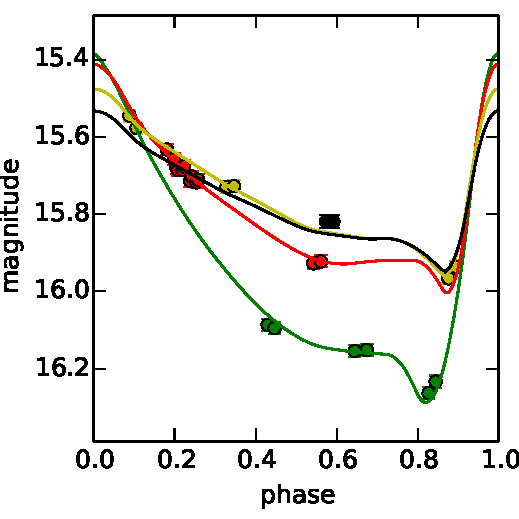
\includegraphics[width=0.5\hsize,clip]{LCniceRR1.pdf}
\caption{An example of a good fit for a known (bright) \RR.} 
\label{Fig:LC1}
\end{figure}


\begin{figure}[!t]
\vskip -0.4in
\hskip 1.3in
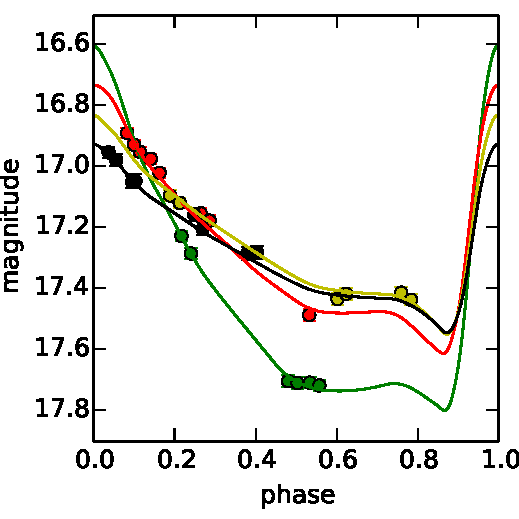
\includegraphics[width=0.5\hsize,clip]{LCniceRR2.pdf}
\caption{An example of a good fit for a known (intermediate brightness) \RR.} 
\label{Fig:LC2}
\end{figure}



\begin{figure}[!t]
\vskip -0.2in
\hskip 1.3in
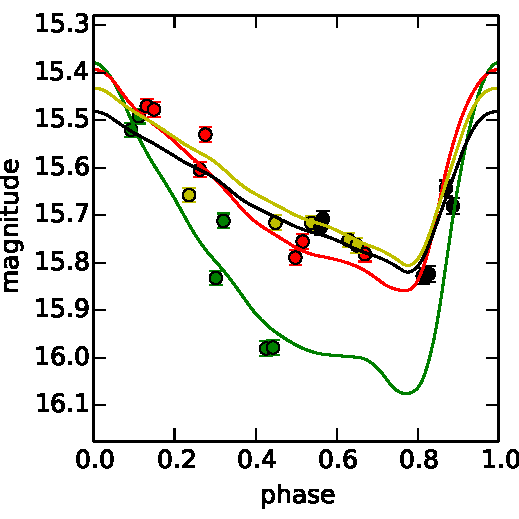
\includegraphics[width=0.5\hsize,clip]{LCbadRR2.pdf}
\caption{An example of a bad fit for a known \RR.} 
\label{Fig:LC3}
\end{figure}


\begin{figure}[!t]
\vskip -0.4in
\hskip 1.3in
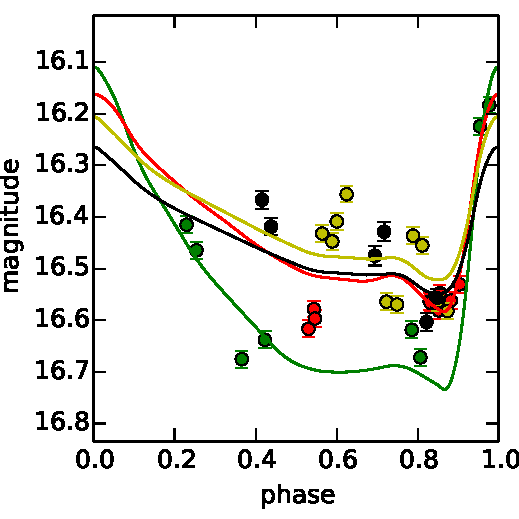
\includegraphics[width=0.5\hsize,clip]{LCbadRR1.pdf}
\caption{An example of a bad fit for a known \RR.} 
\label{Fig:LC4}
\end{figure}


\begin{figure}[!t]
\vskip -0.2in
\hskip 1.3in
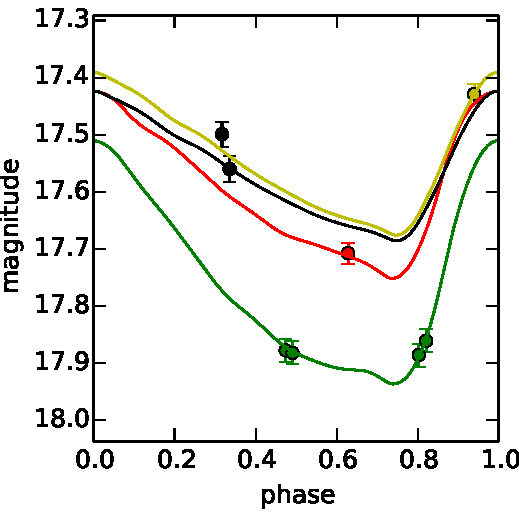
\includegraphics[width=0.5\hsize,clip]{LCgoodOther1.pdf} 
\caption{An example of a good fit for Other subsample.} 
\label{Fig:LC5}
\end{figure}


\begin{figure}[!t]
\vskip -0.4in
\hskip 1.3in
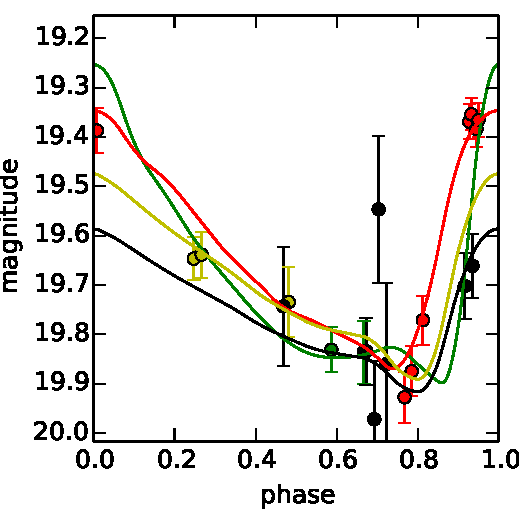
\includegraphics[width=0.5\hsize,clip]{LCgoodOther2.pdf}
\caption{An example of a good fit for Other subsample.} 
\label{Fig:LC6}
\end{figure}



\begin{figure}[!t]
%\vskip -2.5in
\hskip 0.4in
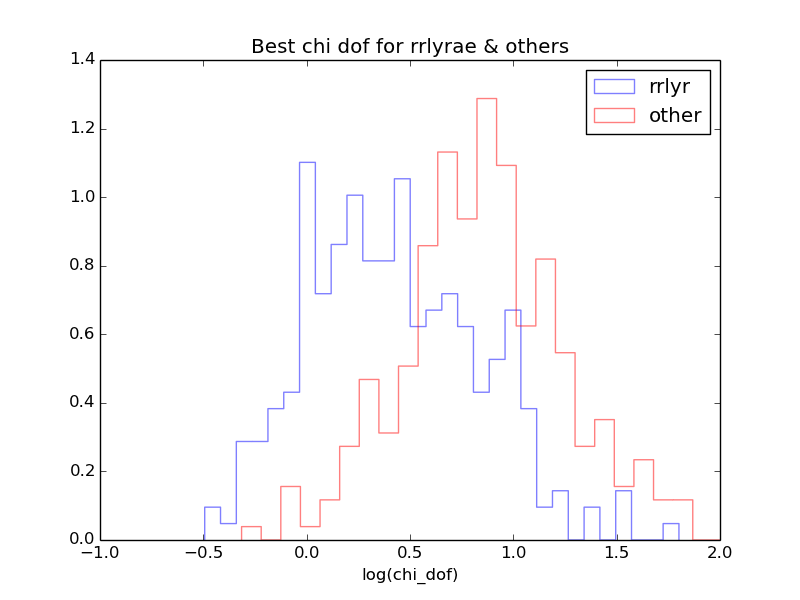
\includegraphics[width=0.9\hsize,clip]{chi2dof.png}
\caption{The distribution of $\chi^2_{dof}$ for known \RR\ (blue) and ``Other'' candidates (red). } 
\label{Fig:chi2dof}
\end{figure}


\begin{figure}[!t]
%\vskip -2.5in
\hskip 0.4in
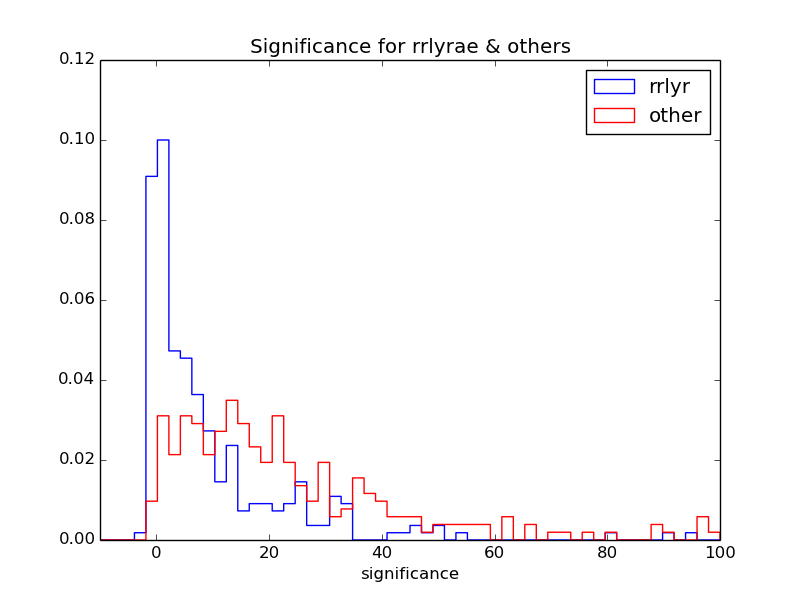
\includegraphics[width=0.9\hsize,clip]{significance.png}
\caption{The distribution of the significance factor, $(\chi^2_{dof}-1) \sqrt{N_{dof}/2}$, for 
known \RR\ (blue) and ``Other'' candidates (red).} 
\label{Fig:sign}
\end{figure}



\begin{figure}[!t]
%\vskip -2.5in
\hskip 0.4in
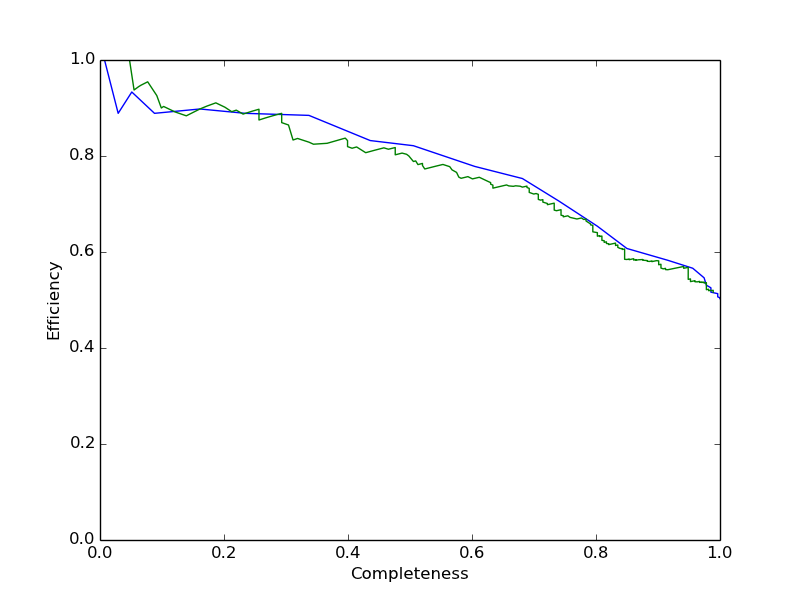
\includegraphics[width=0.9\hsize,clip]{ROC.png}
\caption{The blue curve shows the efficiency vs. completeness (ROC) curve for a classification based 
on $\chi^2_{dof}$. The completeness is relative to the template fitting method (the starting completeness 
is 75\%). The green curve shows performance based on the significance factor, $(\chi^2_{dof}-1) \sqrt{N_{dof}/2}$.} 
\label{Fig:ROC}
\end{figure}



\begin{figure}[!t]
%\vskip -2.5in
\hskip 0.4in
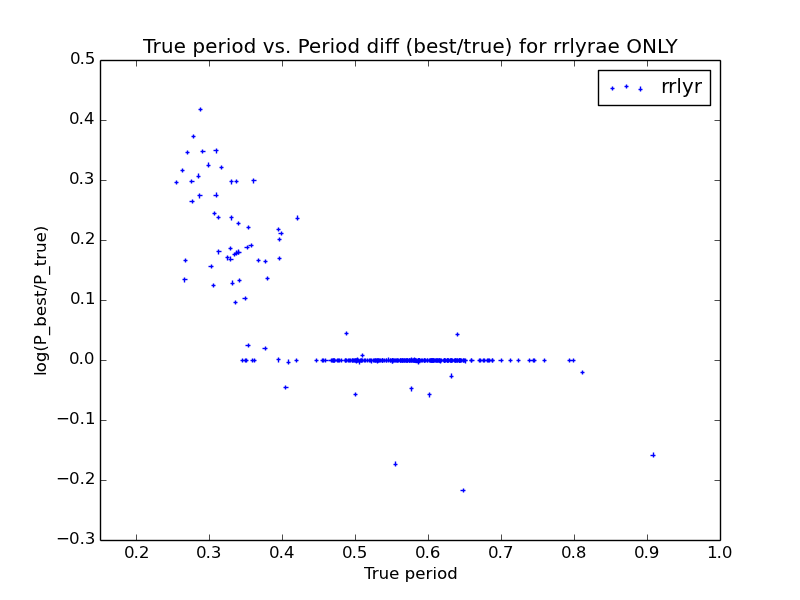
\includegraphics[width=0.9\hsize,clip]{PratPtrue.png}
\caption{The period ``correction'' factor vs. the true (SDSS-based) period for known \RR. For the
majority of c type \RR\ with $P_{true} <0.42$ days, the lack of proper c-type  templates resulted in
grossly incorrect periods (by about a factor of 2). A few were able to recover the correct period 
because the template periods are allowed to vary by $\pm$20\%.} 
\label{Fig:PratPtrue}
\end{figure}


\begin{figure}[!t]
%\vskip -2.5in
\hskip 0.4in
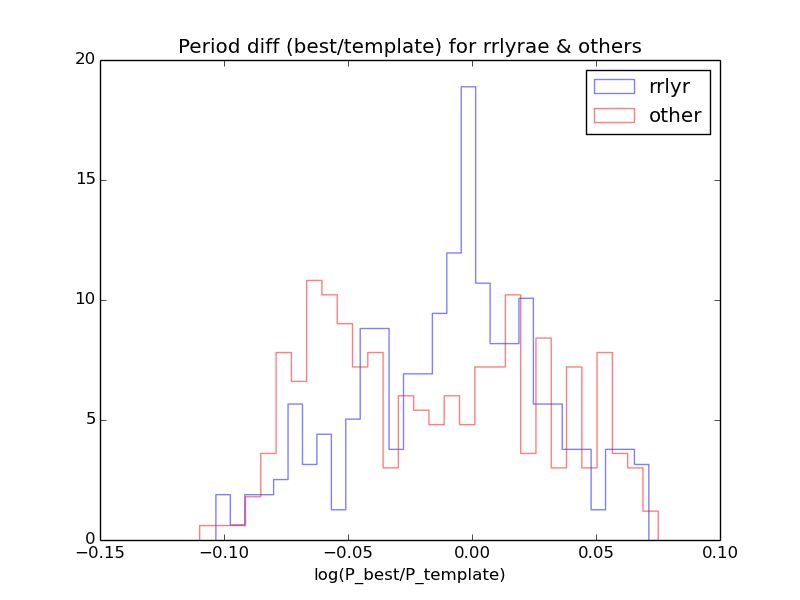
\includegraphics[width=0.9\hsize,clip]{Prat.png}
\caption{The distribution of the period ``correction'' factor for known \RR\ (blue) and ``Other'' candidates (red).} 
\label{Fig:Prat}
\end{figure}




\begin{figure}[!t]
%\vskip -2.5in
\hskip 0.4in
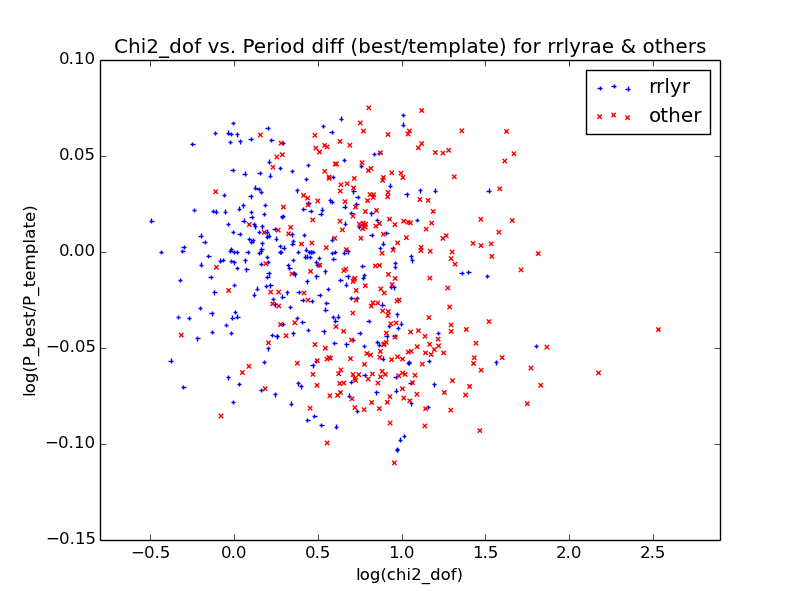
\includegraphics[width=0.9\hsize,clip]{PratChi2.png}
\caption{The period ``correction'' factor vs. $\chi^2_{dof}$ for known \RR\ (blue) and ``Other'' candidates (red).} 
\label{Fig:PratChi2}
\end{figure}



\end{document} 

